\chapter{Modelling the Ionisation Conditions}  \label{chap:Ion-Model}

\section{Ionisation  Modelling}

Relying solely on Voigt profile measurements yields limited information about the absorbers. It gives us the Doppler parameter, which can be used at best to put an upper level on the temperature of the absorbing gas. We need to know the physical conditions underlying in the absorber cloud such as density, temperature, metallicity, etc. As discussed in chapter \ref{chap:intro} that we need to show that the BLA is arising from a collisionally ionised phase, so that we can assure that we are indeed probing the WHIM and not just cool photoionised gas. And by modelling the ionization conditions prevalent in the absorber cloud we can address the aforementioned concerns.

\section{CLOUDY} \label{sec:Cloudy}

To model the ionization conditions prevailing in the absorbers, we use ionization modelling code CLOUDY \citep{cloudy}. CLOUDY considers processes like ionization, recombination, dissociation, and various chemical reactions among atoms, ions, and molecules. These processes determine the composition and abundance of different species in the absorber cloud. CLOUDY accounts for the radiation transfer within the gas cloud. This includes the absorption, emission, and scattering of photons. The simulation considers how radiation interacts with the particles in the cloud, influencing its temperature, density, and ionization state. 

It calculates the ionization equilibrium within the cloud, balancing ionization and recombination processes. It can perform equilibrium calculations for both photoionization and collisional ionization separately and simultaneously as well. To perform photoionization equilibrium calculations we give a model of extragalactic ionization radiation background, which mainly arises from AGNs and star formation activities, whereas for collisional ionization calculations we specify a temperature and then calculations are performed at this constant temperature. A combination of both will give results considering both types of ionizations simultaneously, such models are called hybrid models. 

CLOUDY takes various input parameters like density, temperature, redshift, metallicity of the cloud, abundance pattern of the elements, background radiation model, etc. to perform the equilibrium calculations. It models the clouds as plane parallel slabs with uniform densities and metallicities, and continues to add such slabs until a given stopping criteria is met. As we have the neutral Hydrogen column density from Voigt profile fitting, we use it as stopping criteria for CLOUDY simulations. So CLOUDY continues to add the slabs until the column density of neutral Hydrogen in simulated clouds reaches our given value.
Figure \ref{fig:Cloudy} shows the schematic of a CLOUDY simulation where neutral Hydrogen column density is used as a stopping criteria.
CLOUDY gives us a lot of useful quantities, including column densities and ionization fractions of various ions, equilibrium temperature (for photoionization calculations), etc. We can use these quantities to get the insights on the physical conditions and ionisation state of the absorbers. 

For all the CLOUDY models we set the abundance pattern of elements heavier than Helium to be that of solar abundance as given in \citet{grevesse-chemical-2010} and Helium abundance is set to $8.163\times{10}^{-2}$ (by number relative to Hydrogen) based on the latest CMB measurements \citep{planck_collaboration_planck_2020}. And for extragalactic radiation background model we use KS19 (Q18) model given in \cite{KS19}.  

\begin{figure}[!htbp]
    \centering
    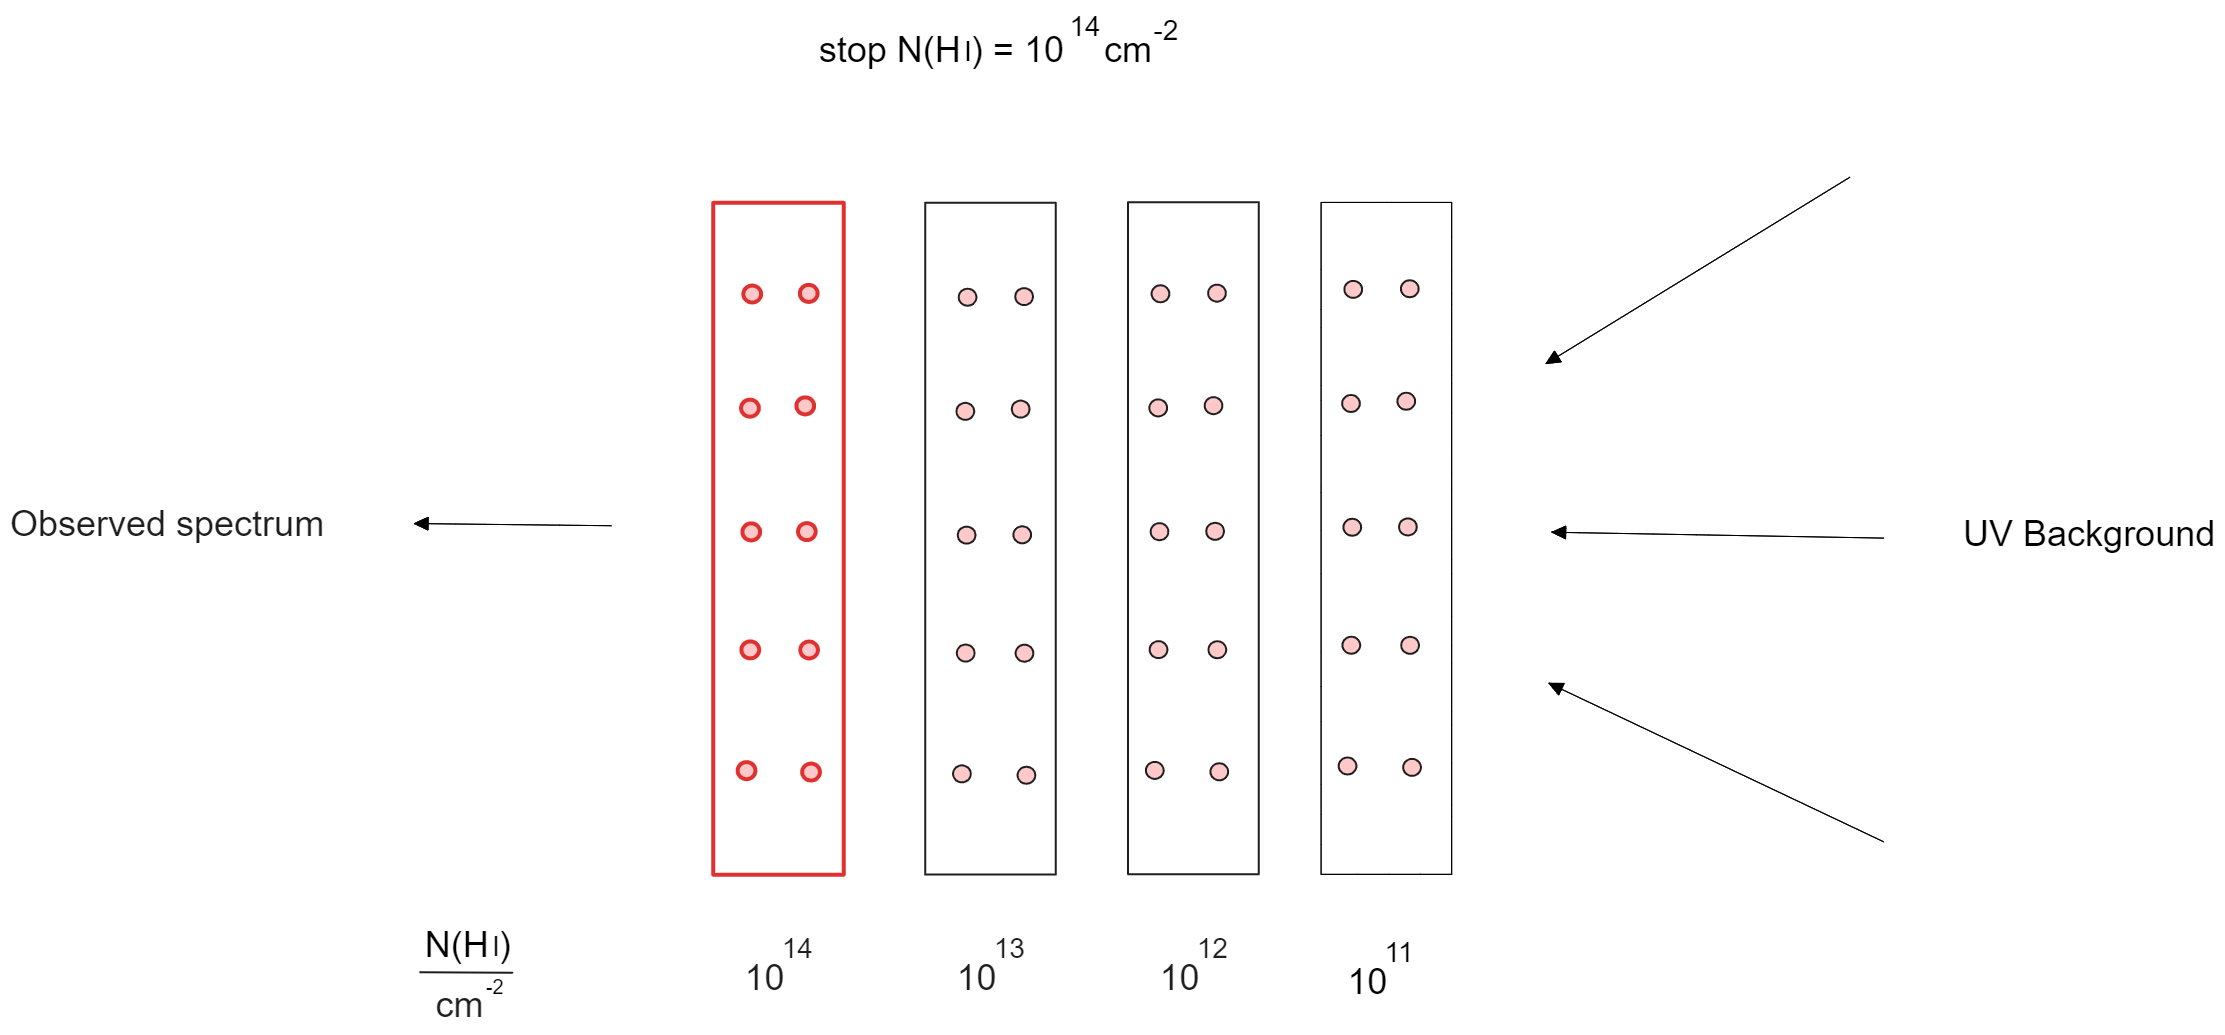
\includegraphics[width=\textwidth]{Figures/Cloudy.png}
    \caption{Schematic of a CLOUDY simulation.}
    \label{fig:Cloudy}
\end{figure}


\section{Ionization Model Based Parameter Estimation}  \label{sec:param-estimation}

As discussed in section \ref{sec:Cloudy}, we use CLOUDY to get the physical conditions existing in the absorber clouds. The physical conditions are characterised by properties like density, temperature, metallicity, pressures, etc. We estimate these quantities based on CLOUDY simulations with methods described in \citet{acharya_khaire}.

We use the $\chi^2$ minimisation technique as discussed in \citet{acharya_khaire} to estimate the density ($n_H$) and metallicity (Z) of the absorber. We consider a dense grid of photoionization CLOUDY models with varying the density ($n_H$) and metallicity (Z) over certain range in the parameter space. We give the  N(\ion{H}{i}) column density from Voigt profile measurements as the stopping criteria for the CLOUDY calculations. We interpolate the column densities in log $n_H$ and log Z space and then use $\chi^2$ minimisation to find the log $n_H$ and log Z values that best fits the data, i.e. the column densities of the observed ions. CLOUDY also gives us the equilibrium temperature also for all the density and metallicity. So we can find the temperature of the absorber cloud by putting the density and metallicity solution which we get from the above procedure. 

In case of collisional ionisation, we can follow the similar approach. If we can get a estimate of the temperature from some other means like using the Doppler parameters of the absorption lines, then we can use the same way of creating a 2D grid of CLOUDY models by fixing the temperature at the known temperature. When we give a constant temperature like this, CLOUDY performs collisional ionisation calculations. And if we don't know the temperature, then we can extend our 2D grid to a 3D one by varying the temperature also. And then use the same approach as in case of 2D grid to find the temperature as well.





